% !TEX root = ../JustinRodriguez-Dissertation.tex

\chapter{Electric field induced metallic behavior in thin crystals of ferroelectric
$\ensuremath{\alpha}\textrm{-In}_{2}\textrm{Se}_{3}$\label{chapter:FeSm-FET}}

<TODO abstract>

\section{Introduction}

Ferroelectric field effect transistors (FeFETs, see \ref{subsec:FeFETs})
are a natural evolution to field effect transistors (FET), providing
a means of maintaining the transistor state without the need for a
constant gate voltage. Typically this is achieved as a standard FET
with a ferroelectric replacing gate dielectric.\citep{si2018ferroelectric,dunkel2017fefet}
Further engineering for use in devices like ferroelectric random access
memory add a metal layer in between the ferroelectric and channel
to enhance the field, and adapt the FinFET design to utilize this
design.\citep{khan2020future} FeFET commercialization, in FRAM and
beyond, still faces many engineering challenges including retention
duration, finding an optimal coercive field and polarization strength,
leakage current through the ferroelectric dielectric, material interface
mismatches, limits to minimization of the ferroelectric.\citep{ma2002why,khan2020future}
With the discovery of conductive ferroelectric compounds, see \ref{subsec:Polar-metals},
we can construct a new variation of the FeFET, where the ferroelectric
acts the role of the semiconductor device channel.\citep{si2018ferroelectric}
Ferroelectric semiconductor field effect transistors (FeSmFETs) opens
up many new possibilities for future devices and may one day answer
the aforementioned obstacles.

In 2017 $\textrm{\ensuremath{\alpha}(3R)-}$ and $\textrm{\ensuremath{\beta}-In}_{2}\textrm{Se}_{3}$
were first predicted to be ferroelectric down to one unit cell.\citep{ding2017prediction}
The $\textrm{\ensuremath{\alpha}-}$phase prediction indicated a combined
binary in-plane (IP) and out-of-plane (OOP) polarization as the selenium
atom shifted in the lattice, while the $\textrm{\ensuremath{\beta}-}$phase
showed only binary IP polarization. Due to the conductive nature of
polar metals it is difficult to preform traditional capacitance-polarization
methods on a crystal as much of the capacitance voltage simply leaks
though the material. In lieu of those measurements many distinct experiments
form a pool of evidence for the existence of ferroelectricity in $\textrm{\ensuremath{\alpha}-In}_{2}\textrm{Se}_{3}$.
Second harmonic generation (SHG) shows a breaking of inversion symmetry\citep{dai2020intrinsic,xiao2018intrinsic,zhou2017outofplane},
a necessary requirement for ferroelectricity. Piezoelectric force
microscopy (PFM) has also shown evidence supporting ferroelectricity\citep{cui2018intercorrelated,wan2018roomtemperature,hou2019resistive,dai2020intrinsic,hou2019ain2se3},
though PFM can often give false positives as similar responses arise
from other phenomena.\citep{vasudevan2017ferroelectric} To counter
this some authors have looked at both IP and OOP PFM response correlation\citep{dai2020intrinsic,hou2019resistive,xiao2018intrinsic,cui2018intercorrelated,liu2019atomically,hou2019ain2se3},
as well as observing the effect IP electric fields to alter the OOP
polarization measured by PFM\citep{hou2019ain2se3}, narrowing the
possibilities of what may be producing false positives.

The largest experimental verification of ferroelectricity in $\textrm{\ensuremath{\alpha}-In}_{2}\textrm{Se}_{3}$
comes from several disparate devices designs that show signs of polarization.
The most explicit example was from an $\textrm{\ensuremath{\alpha}-In}_{2}\textrm{Se}_{3}$/graphene
heterostructure FET. The graphene channel fermi-level shifts from
the electric field produced by the FET gate and the $\textrm{\ensuremath{\alpha}-In}_{2}\textrm{Se}_{3}$
polarization, forming two peaks in the channel resistance as gate
voltage is swept and the fermi-level passes though the charge neutral
point.\citep{wan2019nonvolatile} The authors use this to estimate
a polarization value of 0.92 $\mathrm{\mu C/cm^{2}}$, similar to
the original theoretical prediction of 0.6 $\mathrm{\mu C/cm^{2}}$\citep{ding2017prediction}.
Extensive work has been carried out by multiple group using $\textrm{\ensuremath{\alpha}-In}_{2}\textrm{Se}_{3}$
to create IP\citep{dai2020intrinsic,cui2018intercorrelated,hou2019resistive}
and OOP\citep{wan2018roomtemperature,yang2019nonvolatile} rectifying
devices. For $V_{DS}$ sweeps below the coercive field threshold,
the devices act as a typical semiconductor channel. Above the threshold
voltage the device current shows a significant change in slope, and
a large hysteresis between increasing and decreasing voltage sweeps,
see figure \ref{fig:In2Se3-SampleA-I_DSvV_DS}c and f. Finally, the
recent pioneering of the first FeSmFET using thin crystals of$\textrm{\ensuremath{\alpha}-In}_{2}\textrm{Se}_{3}$
with gate dielectric of 90-nm-thick $\mathrm{SiO_{2}}$ or 15-nm-thick
$\mathrm{HfO_{2}}$. When gated, the channel current showed a large
hysteresis, forming clockwise and counterclockwise loops with the
respective gate dielectric, and persisting down to liquid helium temperatures.\citep{si2019ferroelectric}
Below we discuss the manufacture and measurement of similar $\textrm{\ensuremath{\alpha}-In}_{2}\textrm{Se}_{3}$
FeSmFET devices that show a metallic transition when gated though
a $\mathrm{SiO_{2}}$ dialectic.

\section{Device fabrication}

Thin crystals of $\textrm{\ensuremath{\alpha}-In}_{2}\textrm{Se}_{3}$
were grown by a modified Bridgman method. Transport measurements were
carried out on both bulk and thin mechanically-exfoliated crystals.
For bulk resistivity measurements, silver paint was used to form conductive
terminals. In-plane resistivity measurements were carried out using
a hall bar pattern along the longest axis of the bulk crystal. For
out-of-plane measurements, to ensure a fresh surface, the previous
leads were removed with a razor before new leads were added on. A
modified four-point pattern was used to accommodate the thin c-axis
of the crystal: a current lead was placed in the center of the crystal
on the opposing sides of the c-axis with a voltage lead encircling
each current lead. 

Flakes of thin crystals of $\textrm{\ensuremath{\alpha}-In}_{2}\textrm{Se}_{3}$
on $\textrm{Si:P/Si}\textrm{O}_{2}$ were manufactured using mechanical
exfoliation as described in \ref{subsec:Mechanical-flake-exfoliation}.
Flakes were identified using an optical microscope and atomic force
microscopy was used to establish a rough microscope color code to
judge the thickness of the flakes. Below 20nm, flakes hue was unchanged
but appeared increasingly transparent as thickness decreased. To promote
better van der Walls adhesion of the flake to the substrate, the latter
was first cleaned in Nanostrip, Acetone, 2-Proponal, and DI-water,
before flake exfoliation, and the substrate was heated to 100C while
in contact with the tape prior to the final removal. After optical
identification, flake-substrates were kept in a drybox, or later in
vacuum, to avoid water contamination and oxidation. 

\noindent 
\begin{figure}
\begin{centering}
\subfloat[Hall bar schematic]{\begin{centering}
\includegraphics{Chapter-In2Se3-FeSm-FET/Figures/Hall_bar}
\par\end{centering}
}
\par\end{centering}
\begin{centering}
\subfloat[Sample A]{\includegraphics[width=1.35in]{Chapter-In2Se3-FeSm-FET/Figures/JR200115_11}

}~~~\subfloat[Sample B]{\includegraphics[width=1.35in]{Chapter-In2Se3-FeSm-FET/Figures/JR200115_17}}~~~\subfloat[Sample C]{\includegraphics[width=1.35in]{Chapter-In2Se3-FeSm-FET/Figures/JR190919_03}}~~~\subfloat[Sample D]{\includegraphics[width=1.35in]{Chapter-In2Se3-FeSm-FET/Figures/JR190815_04}}
\par\end{centering}
\caption{Device images\label{fig:In2Se3-Device-images}}

(a) Schematic of the Hall bar device with used in flake measurements,
samples A and B had connected voltage leads for four-point measurements
while C and D had separated leads for hall measurements. (b-e) Optical
images of sample devices following this design with 10 $\mu m$ scale
bars.
\end{figure}

\noindent 
\begin{table}
\begin{centering}
\begin{tabular}{|c|c|c|c|c|c|}
\hline 
Sample & $t\,(nm)$ & $L_{volt}\,\left(\mu m\right)$ & $L_{current}\,\left(\mu m\right)$ & $w\,\left(\mu m\right)$ & Device pattern\tabularnewline
\hline 
\hline 
A & 20 & 2 & 12 & 5 & four-point probe\tabularnewline
\hline 
B & 13 & 4 & 16 & 30 & four-point probe\tabularnewline
\hline 
C & 110 & 5 & 15 & 10 & Hall bar\tabularnewline
\hline 
D & 110 & 2 & 12 & 9 & Hall bar\tabularnewline
\hline 
\end{tabular}
\par\end{centering}
\caption{Device parameters\label{tab:In2Se3-Device-parameters}}

Physical dimensions of the $\ensuremath{\alpha}\textrm{-In}_{2}\textrm{Se}_{3}$
crystals used in the sample devices and the lead configuration. $L_{volt}$
and $L_{current}$ are the distance between the respective voltage
and current leads, $w$ the channel width of the crystal, and $t$
the thickness of the crystal. 
\end{table}

Flakes of crystal were made into four-point probe and Hall bar FET
devices using photolithography and e-beam metal deposition. Similar
to many other van der Waals chalcogenide materials, $\textrm{In}_{2}\textrm{Se}_{3}$
is sensitive to the alkali (base) developers used in many photodevelopment
processes.\citep{choi2011su8,choi2008protective} Initial Hall bar
devices with thinner crystal flakes were completely inoperative after
manufacture, while thicker devices showed substantial Schottky barriers
on various contacts. Milling away crystal material between the lithography
and metal evaporation produced better contacts, but inconstantly,
and only worked with thicker devices. To circumvent this effect, we
modified our lithography step to only allow solvent developers in
contact with the flake material, with the procedure described in section
\ref{subsec:PMMA+PMGI+SPR}. 5 nm of titanium and 45 nm of gold was
evaporated using either a Lab-18 Thin Film Deposition System (Kurt
J. Lesker Co.) or a Temescale FC2000 (Ferrotec). The excess material
was removed using the solvent Remover-PG (Microchem). Figure \ref{fig:In2Se3-Device-images}
shows the layout and optical images of the devices measured in this
chapter, table \ref{tab:In2Se3-Device-parameters} the corresponding
parameters of those devices. All measurements were carried out in
low vacuum, less than 1 mTorr, in a Model 6000 Physical Properties
Measurement System (PPMS, Quantum Design). A Keithley 6340 was used
as the current and voltage bias source as well as the corresponding
two-point voltage and current measurements, two Keithley 2182A were
used for four-point and hall measurements across the voltage leads,
and a Keithley 2400 was used to provide the gate voltage bias.

\section{Optical characterization of the $\textrm{\ensuremath{\alpha}-In}_{2}\textrm{Se}_{3}$
crystal flakes}

Indium and selenium can form a variety of compounds, and the growth
process is complicated and may result in crystals with mixed polymorphs,
see section \ref{subsec:In-Se-compounds}.\citep{liu2019atomically}
Because of this, several optical measurements were used to confirm
the stoichiometry and lattice stacking of the material used in our
devices. X-Ray diffraction measurements displayed peaks corresponding
to the $R3m$ or $R\bar{3}m$ space groups, indicating $\alpha$-
or $\beta$-phase. Raman showed peaks near 104, 179, and 193 $cm^{-1}$corresponding
to the $A_{1}^{\,1}$, $E^{3}$, and $A_{1}^{\,4}$ peaks of $\textrm{\ensuremath{\alpha}-In}_{2}\textrm{Se}_{3}$.\citep{liu2019atomically,balakrishnan2018epitaxial}
Photoluminescence showed an energy gap of 1.4 $eV$, consistent with
previous $\textrm{\ensuremath{\alpha}-In}_{2}\textrm{Se}_{3}$ optical
measurements.\citep{balakrishnan2018epitaxial} Finally, angle-resolved
SHG showed a six-fold symmetry establishing the material as stacking
in a $R3m$ (166) space group lattice.\citep{hou2019resistive,dai2020intrinsic,xiao2018intrinsic}
Figure \ref{fig:In2Se3-Optical-measurements} shows the Raman, photoluminescence,
and SHG measurements performed on exfoliated flakes of crystal on
$\textrm{Si:P/Si}\textrm{O}_{2}$ wafer chips. Raman and photoluminescence
measurements were taken using a Renishaw inVia Raman microscope (488
nm laser).

\noindent 
\begin{figure}
\begin{centering}
\subfloat[Raman]{\begin{centering}
\includegraphics[width=0.3\textwidth]{\string"Chapter-In2Se3-FeSm-FET/Figures/In2Se3_Raman - F2-P1-60s_2times_10per160uW_x100_r\string".pdf}
\par\end{centering}
}\hspace*{\fill}\subfloat[Photoluminescence]{\centering{}\includegraphics[width=0.3\textwidth]{\string"Chapter-In2Se3-FeSm-FET/Figures/In2Se3_Photoluminescence - F2-P2-60s_2times_10per160uW_x100_pl\string".pdf}}\hspace*{\fill}\subfloat[Angle-resolved SHG]{\begin{centering}
\includegraphics[width=0.3\textwidth]{\string"Chapter-In2Se3-FeSm-FET/Figures/In2Se3_angled_SHG - In2Se3_SiO2Si_03262019_pol_5mW_50xLWD_55NA_1000ms_100umslit_1_1\string".pdf}
\par\end{centering}
}\caption{Optical measurements of $\textrm{\ensuremath{\alpha}-In}_{2}\textrm{Se}_{3}$.\label{fig:In2Se3-Optical-measurements} }
\par\end{centering}
Raman <TODO peak numbers> (a), photoluminescence (b), and angle-resolved
SHG (c) of exfoliated $\textrm{\ensuremath{\alpha}-In}_{2}\textrm{Se}_{3}$
flakes on Si-$\mathrm{SiO_{2}}$substrate.
\end{figure}


\section{FET measurements}

Thin crystals of $\textrm{\ensuremath{\alpha}-In}_{2}\textrm{Se}_{3}$
were manufactured into Hall bar and four-point probe FETs. Devices
were made on conductive substrates of doped silicon with an insulating
layer of 300nm thermally grown $\textrm{Si:P/Si}\textrm{O}_{2}$,
allowing us to use the substrate as the gate in the FETs. Figure \ref{fig:In2Se3-SampleA-I_DSvV_DS}
shows sample A source-drain current $I_{D}$ measured against voltage
bias $V_{DS}$ from 0 to 5 V, and separately for 0 to -5 V, for fixed
back gate voltages. Gate voltages were fixed in 25 V intervals from
-75 V to 75 V for each sequence. The rapid increase in $I_{D}$ at
low voltages is indicative of two back-to-back Schottky diodes, see
section \ref{sec:Metal-Semiconductor-Metal-conduc}. Samples B and
C showed a similar measurement with both the increasing and decreasing
$V_{DS}$ bias for fixed gate voltages, figures \ref{fig:Sample-B-IDvsVDS-log}
and \ref{fig:Sample-C-IDvsVDS-log}. None of the samples measured
were seen to saturate within $\pm10$ V for any gate bias. The lower
$I_{D}$ for negative $V_{DS}$ bias than positive is typical of n-type
semiconductors, which is seen in most reports of $\textrm{\ensuremath{\alpha}-In}_{2}\textrm{Se}_{3}$\citep{island2015gate,julien1986electrical}.
Sample A $V_{DS}$ was cycled from 0 V, 10 V, -10V, to 0 V, forming
asymmetric hysteresis in the current. The switching behavior is similar
to previous reports of $\textrm{\ensuremath{\alpha}-In}_{2}\textrm{Se}_{3}$
rectifying devices, where the ferroelectric polarization field is
thought to modify the Schottky barrier between the material and the
metal leads.\citep{yang2019nonvolatile,wan2018roomtemperature,cui2018intercorrelated,dai2020intrinsic}
The increasing drain current with positive gate voltages is indiciative
of a $n$-type semiconductor\citep{horowitz2015art}, consistent with
previous measurements on $\textrm{\ensuremath{\alpha}-In}_{2}\textrm{Se}_{3}$\citep{julien1986electrical,island2015gate}.

\noindent 
\begin{figure}
\begin{centering}
\subfloat[$I_{D}\left(V_{DS,\uparrow},\,V_{G,\uparrow}\right)$]{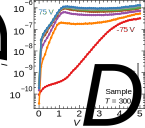
\includegraphics[width=5cm]{Chapter-In2Se3-FeSm-FET/Figures/JR200115_11/JR200115_11_300K_IDvVDS-positive_VG-increasing_log_txt}}~~\subfloat[$I_{D}\left(V_{DS,\downarrow},\,V_{G,\uparrow}\right)$]{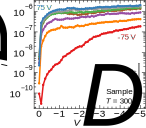
\includegraphics[width=5cm]{Chapter-In2Se3-FeSm-FET/Figures/JR200115_11/JR200115_11_300K_IDvVDS-negative_VG-increasing_log_txt}}~~\subfloat[$I_{D}\left(V_{DS,\updownarrow},\,V_{G,\uparrow}\right)$]{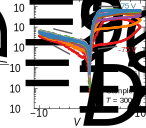
\includegraphics[width=5cm]{Chapter-In2Se3-FeSm-FET/Figures/JR200115_11/JR200115_11_300K_IDvVDS-loop_VG-increasing_log_txt}

}
\par\end{centering}
\noindent \begin{centering}
\subfloat[$I_{DS}\left(V_{DS,\uparrow},\,V_{G\downarrow}\right)$]{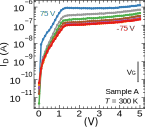
\includegraphics[width=5cm]{Chapter-In2Se3-FeSm-FET/Figures/JR200115_11/JR200115_11_300K_IDvVDS-positive_VG-decreasing_log_txt}}~~\subfloat[$I_{D}\left(V_{DS,\downarrow},\,V_{G,\downarrow}\right)$]{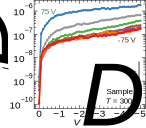
\includegraphics[width=5cm]{Chapter-In2Se3-FeSm-FET/Figures/JR200115_11/JR200115_11_300K_IDvVDS-negative_VG-decreasing_log_txt}}~~\subfloat[$I_{D}\left(V_{DS,\updownarrow},\,V_{G,\downarrow}\right)$]{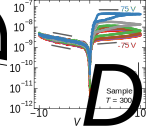
\includegraphics[width=5cm]{Chapter-In2Se3-FeSm-FET/Figures/JR200115_11/JR200115_11_300K_IDvVDS-loop_VG-decreasing_log_txt}

}\caption{Sample A: $I_{D}\left(V_{DS}\right)$\label{fig:In2Se3-SampleA-I_DSvV_DS}}
\par\end{centering}
$I_{D}\left(V_{DS}\right)$ of sample A with positive-increasing (a
\& d) and negative-decreasing (b \& e) $V_{DS}$. (c \& f) hysteresis
in $I_{D}$ as $V_{DS}$ is cycled from 0 V, 10 V, -10 V, to 0 V.
Measurements (a - c) are taken while $V_{G}$ is held at 25 V intervals
that increase sequentially for each curve, and (d - f) decreasing
for $V_{G}$ intervals. All measurements were done at 300 K.
\end{figure}

FET transistor transfer curves, current as a function of gate voltage
$V_{G}$, were measured for each device. All measurements shown were
performed with a fixed $V_{DS}=.1V$, with the $V_{G}$ cycled from
0 V, to -75 V, 75 V, -75 V, to 0 V, shown in figure \ref{fig:In2Se3-Sample-A-loops}.
For clarity, only the data between -75 V, 75 V, to -75 V is shown,
as that behavior is persistent across multiple loops. The measurement
was repeated at various, fixed temperatures from 300 K to 2-4 K, the
lowest temperature reached is sample dependent due to ice blockages
in the PPMS cooling. For each gate voltage sweep sweep the current
formed a clockwise hysteresis loop. In all samples the width of the
loop decreased with decreasing temperature, though each sample still
exhibited a finite hysteresis at the lowest temperature. Samples B
and C showed similar clockwise hysteresis behavior, shown in \ref{fig:Sample-B-loops}
and \ref{fig:Sample-C-loops}. This behavior is consistent with previous
work with $n$-type $\textrm{\ensuremath{\alpha}-In}_{2}\textrm{Se}_{3}$
on $\textrm{Si}\textrm{O}_{2}$ FeSmFETs.\citep{si2019aferroelectric} 

\noindent 
\begin{figure}
\begin{centering}
\subfloat[300 K]{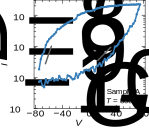
\includegraphics[width=5cm]{Chapter-In2Se3-FeSm-FET/Figures/JR200115_11/JR200115_11_IDvVG_300K_log_txt}}~~\subfloat[200 K]{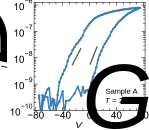
\includegraphics[width=5cm]{Chapter-In2Se3-FeSm-FET/Figures/JR200115_11/JR200115_11_IDvVG_200K_log_txt}}~~\subfloat[150 K]{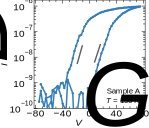
\includegraphics[width=5cm]{Chapter-In2Se3-FeSm-FET/Figures/JR200115_11/JR200115_11_IDvVG_150K_log_txt}

}
\par\end{centering}
\begin{centering}
\subfloat[100 K]{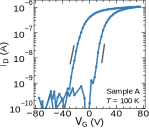
\includegraphics[width=5cm]{Chapter-In2Se3-FeSm-FET/Figures/JR200115_11/JR200115_11_IDvVG_100K_log_txt}}~~\subfloat[50 K]{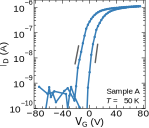
\includegraphics[width=5cm]{Chapter-In2Se3-FeSm-FET/Figures/JR200115_11/JR200115_11_IDvVG_050K_log_txt}}~~\subfloat[2 K]{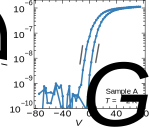
\includegraphics[width=5cm]{Chapter-In2Se3-FeSm-FET/Figures/JR200115_11/JR200115_11_IDvVG_002K_log_txt}

}
\par\end{centering}
\begin{centering}
\caption{Sample A: $I_{D}\left(V_{G}\right)$ transfer characteristics\label{fig:In2Se3-Sample-A-loops}}
\par\end{centering}
$I_{D}\left(V_{G}\right)$ of sample A at the indicated fixed temperatures.
Each was measured with $V_{DS}=0.1\,V$ as $V_{G}$ was cycled, a
clockwise hysteresis current loop was seen at all temperatures.
\end{figure}


\section{Discussion (TODO: add?, review)}

\begin{figure}
\begin{centering}
\subfloat[Bulk: $\rho\left(T\right)$]{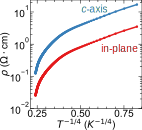
\includegraphics[width=5cm]{Chapter-In2Se3-FeSm-FET/Figures/In2Se3_Bulk_RT_ln}

}~~~\subfloat[Sample A: $R_{DS}\left(T\right)$]{~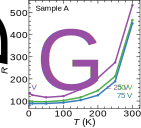
\includegraphics[width=4.95cm]{Chapter-In2Se3-FeSm-FET/Figures/JR200115_11/JR200115_11_RDSvVG-cross-section_linear}}
\par\end{centering}
\begin{centering}
\subfloat[Sample B: $R_{DS}\left(T\right)$]{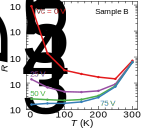
\includegraphics[width=5cm]{Chapter-In2Se3-FeSm-FET/Figures/JR200115_17/JR200115_17_RDSvVG-cross-section_log}}~~~\subfloat[Sample C: $R_{DS}\left(T\right)$]{~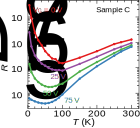
\includegraphics[width=5cm]{Chapter-In2Se3-FeSm-FET/Figures/JR190919_03/JR190919_03_RDSvVG-cross-section_log}

}
\par\end{centering}
\caption{Temperature dependence\label{fig:Temperature-dependence}}

(a) Bulk crystal resistivity along the c-axis and in-plane. (b-d)
Temperature cross-section of the $I_{D}\left(V_{G}\right)$ transfer
characteristics for samples A, B, and C for the curves shown in figures
\ref{fig:In2Se3-Sample-A-loops}, \ref{fig:Sample-B-loops}, and \ref{fig:Sample-C-loops}
respectively. Each data-point is taken from the increasing $V_{G}$
(top) portion of the respective $I_{D}\left(V_{G}\right)$ curves
for 0, 25, 50, and 75 V.
\end{figure}

When cooled from 300 to 2 K, the $\textrm{\ensuremath{\alpha}-In}_{2}\textrm{Se}_{3}$
bulk crystal showed an increase in resistivity emblematic of most
semiconductors, seen in figure \ref{fig:Temperature-dependence}a,
with variable range hopping conduction appearing below approximately
40 K. In contrast thin gated crystals of $\textrm{\ensuremath{\alpha}-In}_{2}\textrm{Se}_{3}$showed
a more positive $dR/dT$ slope for increasing positive gate voltages.
Figure \ref{fig:Temperature-dependence}b-d show a cross section of
the $I_{D}\left(V_{G}\right)$ transport measurements taken at different
temperatures of samples A, B, and C, shown in figures \ref{fig:In2Se3-Sample-A-loops},
\ref{fig:Sample-B-loops}, and \ref{fig:Sample-C-loops}. $V_{G}=0$
shows a similar behavior to the bulk crystal, while 50 V and 75 V
have a $dR/dT$ slope indicative of a metallic state. The cross section
of $I_{D}\left(V_{G}\right)$ is used to examine the metallic transition
of the devices as the increased conductivity state was quickly destroyed
with changing temperatures, and was sensitive to the previous state
of the system, see figure \ref{fig:Sample-C-effects-of-warming-cooling}.
In all samples the onset of the uptick in conductivity occurs at higher
voltages as temperatures decrease, leading to a shrinking but finite
hysteresis loop. These behaviors seem to be independent of ramping
rate of $V_{G}$ ($\ref{fig:Sample-B-rate-dependance}$) and contact
resistance does not appear to play a significant role in sample resistance
(figures \ref{fig:Sample-C-effects-of-warming-cooling} and \ref{fig:Sample-D-contact-resistance}).

The magnetoconductance (MC) of sample A displayed weak localization
while gated into the metallic state at 1.8 K (figure \ref{fig:Magnetic-field-measurment}d),
as well as 10 and 50 K (figure \ref{fig:Sample-A:-magnetoconductance-All-K}).
The MC data was quantitatively fit to the Hikami-Larkin-Nagaoka theory
of 2D weak localization, equation \ref{eq:Hikami-Larkin-Nagaoka}
discussed in section \ref{subsec:Weak-localization}. The fit quality
decreases significantly with increasing temperature, as might be expected
with the lessening of the localization, shown in table \pageref{tab:Sample-A:-magnetoconductance}.
All temperatures show similar mean free paths of phase coherence $l_{\phi}$
and elastic scattering $l_{e}$, much smaller than the spin-orbit
coupling $l_{SO}$. Sample C shows a small uptick in cross-section
resistance near liquid helium temperatures, this is likely a result
of disorder in the sample C crystal. Weak localization in a 2D system
can manifest a non-metallic, negative $dR/dT$ at low temperatures\citep{lee1985disordered},
which is consistent with what we observed.

\noindent 
\begin{figure}
\begin{centering}
\subfloat[Sample A:\protect \\
\qquad{}magnetoconductance fit]{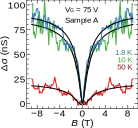
\includegraphics[width=5cm]{Chapter-In2Se3-FeSm-FET/Figures/JR200115_11/JR200115_11_Magnetoconductance_All-K_fit}}~~\subfloat[Sample D:\protect \\
\qquad{}Carrier density $n_{2D}\left(T\right)$]{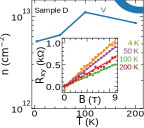
\includegraphics[width=5cm]{Chapter-In2Se3-FeSm-FET/Figures/JR190815_04/JR190815_04_Hall_combined}}
\par\end{centering}
\caption{Magnetic field measurements\label{fig:Magnetic-field-measurment}}

(a) The magnetoconductance of sample A taken at 1.8, 10 and 50 K.
The data was symmetrized to remove odd-term magnetic field dependence,
and normalized to the difference from the measured value at zero-field.
The fitting parameters are given in table \ref{tab:Sample-A:-magnetoconductance},
showing a better fit at lower temperatures. (b) Sample D carrier density
at various temperatures, the inset shows the hall data used the the
carrier density calculations.
\end{figure}

\noindent 
\begin{table}
\begin{centering}
\begin{tabular}{|c|c|c|c|c|}
\hline 
 & $l_{\phi}$ & $l_{SO}$ & $l_{e}$ & $r^{2}$\tabularnewline
\hline 
\hline 
1.8 K & 29 nm & 420 nm & 28 nm & 0.937\tabularnewline
\hline 
10 K & 27 nm & 460 nm & 27 nm & 0.820\tabularnewline
\hline 
50K & 29 nm & 140 nm & 28 nm & 0.732\tabularnewline
\hline 
\end{tabular}
\par\end{centering}
\caption{Sample A: magnetoconductance fit parameters\label{tab:Sample-A:-magnetoconductance}}
\end{table}

The $\textrm{\ensuremath{\alpha}-In}_{2}\textrm{Se}_{3}$ sample hysteresis
is likely from combination of charge trapping and the ferroelectric
nature of the material. In FeFETs both charge trapping and polarization
switching can display similar hysteresis behaviors, and care must
be taken when determining the explanation of that hysteresis\citep{kokil2012techniques,yurchuk2016chargetrapping,osullivan2020defect,jung2020impact},
especially with DC measurements. As almost all MOSFET devices show
evidence of charge trapping, even in the long-studied and optimized
Si-$\mathrm{SiO_{2}}$ interface, we can assume it plays some role
in our devices. Additionally, the reported devices were manufactured
within air, adding increased interface contamination from water and
air\citep{datye2018reduction,bartolomeo2017hysteresis,kim2018analysis}.
In FETs we expect to see a reduction in charge trapping hysteresis
in $I_{D}$-$V_{G}$ sweeps with decreasing temperature\citep{datye2018reduction,kim2018analysis,park2021interface,bartolomeo2017hysteresis,guo2015charge},
though the effects of charge traps can still be seen even down to
cryogenic temperatures\citep{liu2021cryogenic,beckers2020physical,park2021interface,beckers2018cryogenic,powell1983charge}.
All of the reported devices showed a similar reduction in the size
of the hysteresis gate voltage widths with decreasing temperature,
shown in figure \ref{fig:dVG-vs-T} for various currents. In FeFET
devices we would expect an increasing hysteresis window at lower temperature
from the suppressed charge trapping effects\citep{wang2020cryogenic,ni2018critical,ali2020study},
reduced domain wall motion\citep{tan2020hot}, or a change in polarization
and coercive fields\citep{ali2020study}. As the role of ferroelectricity
in the semiconductor and dielectric are the switched in a FeSmFET
verses a traditional FeFET, the interactions between charge traps
dipoles are not the same as in a traditional FeFET. More work is needed
to quantify the agency of the hysteresis behavior.

The mechanism responsible for the $\textrm{\ensuremath{\alpha}-In}_{2}\textrm{Se}_{3}$
metallic state has many possible explanations. The origin metal-insulator-transitions
(MIT) in MOSFETs is still an area active study\citep{moon2021metalinsulator},
but current theories generally fall under carrier-carrier interactions,
disorder scattering, or some combination of the two. Of the former,
one of the most prevalent is the prediction that in 2D semiconductor
TMDs, carrier-carrier interactions cause a Wigner-Mott transition\citep{amaricci2010extended,moon2021metalinsulator,moon2020quantum}.
In a Mott insulator carriers localize to form spin 1/2 bound states
in the potential wells of Coulomb repulsion from surrounding carriers,
and at increased carrier density the carriers overcome the repulsion
and form a Fermi liquid. A second common suggestion is that MITs may
result from percolation in layered semiconductors\citep{moon2019anomalous,tracy2009observation,moon2021metalinsulator,manfra2007transport,dassarma2005twodimensional}.
In a 2D semiconductor a small change in carrier density leads to a
large change in screening, and at low carrier density and screening
the disorder of the system has a significant impact on the carrier
conduction. Theoretical predictions also have suggested disorder from
charge trapping may also display a metal-to-insulator (MIT) in MOSFETs\citep{brunthaler2007trap,altshuler1999theory,hormann2010dipole}.
See section \ref{subsec:Localization} for a more thorough description
of the aforementioned MITs. From the $I_{D}$-$V_{DS}$ in plane current
sweep hysteresis, typically attributed to domain switching in $\textrm{\ensuremath{\alpha}-In}_{2}\textrm{Se}_{3}$
devices, we may postulate that the ferroelectric nature of the $\textrm{\ensuremath{\alpha}-In}_{2}\textrm{Se}_{3}$
crystal likely plays some role in or interacts with the origin of
the observed metallic state. However, neither the mechanisms for conductivity
in ferroelectric semiconductors<TODO:refs> or the dynamics polarization
will play in a FET configuration<TODO:refs> are well understood. Additionally,
with only one experimentally verified ferroelectric metal\citep{zhou2020review},
demonstrated very recently\citep{fei2018ferroelectric,sharma2019roomtemperature},
there has been little study of polarization switching behaviors in
actual ferroelectric metals. FeSmFETs, along with FeFETs\citep{lu2018electrically},
may provide us with a new avenue to understand MITs using ferroelectric
polarization. 

TODO: smooth discussion transition

TODO: Include discussion on max 2D electric conductivity? No idea
where the 80$\sigma_{0}$ (quantum conductance) for Prof Liu's calculation
comes from. I get .1-.2$\sigma_{0}$ for thick samples and \textasciitilde 2.5$\sigma_{0}$
for thin ones.

TODO: Discuss ferroelectric channel conduction? Finish background
discussion on ferroelectric channels/semiconductors first.

TODO: include trapped charge calculation assuming no FE?

TODO: \citep{hu2021firstprinciples}

\section{Future work (TODO)}
\begin{itemize}
\item simulations: In2Se3 has dipole locking. FeSmFETs have not been studied.
Narrow bandgap semiconductor domains
\item PFM measurements showing domain motion during gating, MIT
\item Domain wall conductivity
\item effects of encapsulation on MIT
\end{itemize}

\section{Conclusion (TODO)}

\section{Data from additional samples (TODO: integrate more with above)}

\begin{figure}
\noindent \begin{centering}
\subfloat[$I_{D}\left(V_{DS,\uparrow},\,V_{G,\uparrow}\right)$\hfill{}]{\raggedleft{}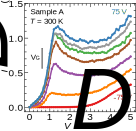
\includegraphics[width=4.75cm]{Chapter-In2Se3-FeSm-FET/Figures/JR200115_11/JR200115_11_300K_IDvVDS-positive_VG-increasing_linear_txt}}~~~\subfloat[$I_{D}\left(V_{DS,\downarrow},\,V_{G,\uparrow}\right)$\hfill{}]{\raggedleft{}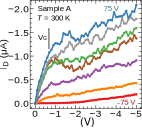
\includegraphics[width=5.04cm]{Chapter-In2Se3-FeSm-FET/Figures/JR200115_11/JR200115_11_300K_IDvVDS-negative_VG-increasing_linear_txt}}~~~\subfloat[$I_{D}\left(V_{DS,\updownarrow},\,V_{G,\uparrow}\right)$]{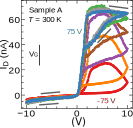
\includegraphics[width=4.66cm]{Chapter-In2Se3-FeSm-FET/Figures/JR200115_11/JR200115_11_300K_IDvVDS-loop_VG-increasing_linear}

}
\par\end{centering}
\noindent \begin{centering}
\subfloat[$I_{D}\left(V_{DS,\uparrow},\,V_{G,\downarrow}\right)$]{\raggedleft{}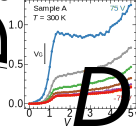
\includegraphics[width=4.85cm]{Chapter-In2Se3-FeSm-FET/Figures/JR200115_11/JR200115_11_300K_IDvVDS-positive_VG-decreasing_linear_txt}}~~\subfloat[$I_{D}\left(V_{DS,\downarrow},\,V_{G,\downarrow}\right)$]{\raggedleft{}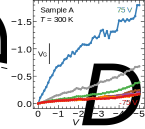
\includegraphics[width=5.13cm]{Chapter-In2Se3-FeSm-FET/Figures/JR200115_11/JR200115_11_300K_IDvVDS-negative_VG-decreasing_linear_txt}}~~\subfloat[$I_{D}\left(V_{DS,\updownarrow},\,V_{G,\downarrow}\right)$]{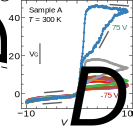
\includegraphics[width=4.8cm]{Chapter-In2Se3-FeSm-FET/Figures/JR200115_11/JR200115_11_300K_IDvVDS-loop_VG-decreasing_linear}

}
\par\end{centering}
\begin{centering}
\caption{Sample A: $I_{D}\left(V_{DS},\,V_{G}\right)$\label{fig:Sample-A-IDvsVDS}}
\par\end{centering}
$I_{D}\left(V_{DS}\right)$ of sample A, linear scaling of data shown
in figure \ref{fig:In2Se3-SampleA-I_DSvV_DS}. (a \& d) Show positive-increasing
$V_{DS}$ and (b \& e) negative-decreasing $V_{DS}$. (c \& f) hysteresis
in $I_{D}$ as $V_{DS}$ is cycled from 0 V, 10 V, -10 V, to 0 V.
Measurements (a - c) are taken while $V_{G}$ is held at 25 V intervals
that increase sequentially for each curve, and (d - f) decreasing
for $V_{G}$ intervals. All measurements were done at 300 K.
\end{figure}

\noindent 
\begin{figure}
\begin{centering}
\subfloat[$I_{D}\left(V_{DS,\uparrow},\,V_{G,\uparrow}\right)$\hfill{}]{\raggedleft{}%
\begin{minipage}[t]{0.3\paperwidth}%
\begin{flushright}
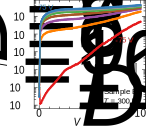
\includegraphics[width=5cm]{Chapter-In2Se3-FeSm-FET/Figures/JR200115_17/JR200115_17_300K_IDvVDS-positive_VG-increasing_log_txt}\qquad{}
\par\end{flushright}%
\end{minipage}}\quad{}\subfloat[$I_{D}\left(V_{DS,\downarrow},\,V_{G,\uparrow}\right)$\hfill{}]{\raggedleft{}%
\begin{minipage}[t]{0.3\paperwidth}%
\begin{flushright}
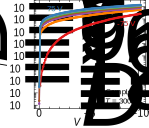
\includegraphics[width=5cm]{Chapter-In2Se3-FeSm-FET/Figures/JR200115_17/JR200115_17_300K_IDvVDS-negative_VG-increasing_log_txt}\qquad{}
\par\end{flushright}%
\end{minipage}}
\par\end{centering}
\begin{centering}
\subfloat[$I_{D}\left(V_{DS,\uparrow},\,V_{G,\downarrow}\right)$]{\raggedleft{}%
\begin{minipage}[t]{0.3\paperwidth}%
\begin{flushright}
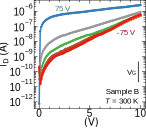
\includegraphics[width=5cm]{Chapter-In2Se3-FeSm-FET/Figures/JR200115_17/JR200115_17_300K_IDvVDS-positive_VG-decreasing_log_txt}\qquad{}
\par\end{flushright}%
\end{minipage}}\quad{}\subfloat[$I_{D}\left(V_{DS,\downarrow},\,V_{G,\downarrow}\right)$]{\raggedleft{}%
\begin{minipage}[t]{0.3\paperwidth}%
\begin{flushright}
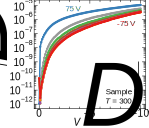
\includegraphics[width=5cm]{Chapter-In2Se3-FeSm-FET/Figures/JR200115_17/JR200115_17_300K_IDvVDS-negative_VG-decreasing_log_txt}\qquad{}
\par\end{flushright}%
\end{minipage}}
\par\end{centering}
\begin{centering}
\caption{Sample B: $I_{D}\left(D_{DS},\,V_{G}\right)$ - logarithmic scale\label{fig:Sample-B-IDvsVDS-log}}
\par\end{centering}
$I_{D}\left(V_{DS}\right)$ of sample B with positive-increasing (a
\& c) and negative-decreasing (b \& d) $V_{DS}$. Measurements (a
\& b) are taken while $V_{G}$ is held at 25 V intervals that increase
sequentially for each curve, and (c \& d) decreasing for $V_{G}$
intervals. All measurements were done at 300 K.
\end{figure}

\noindent 
\begin{figure}
\begin{centering}
\subfloat[$I_{D}\left(V_{DS,\uparrow},\,V_{G,\uparrow}\right)$\hfill{}]{\raggedleft{}%
\begin{minipage}[t]{0.3\paperwidth}%
\begin{flushright}
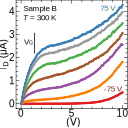
\includegraphics[width=4.37cm]{Chapter-In2Se3-FeSm-FET/Figures/JR200115_17/JR200115_17_300K_IDvVDS-positive_VG-increasing_linear_txt}\qquad{}
\par\end{flushright}%
\end{minipage}}\quad{}\subfloat[$I_{D}\left(V_{DS,\downarrow},\,V_{G,\uparrow}\right)$\hfill{}]{\raggedleft{}%
\begin{minipage}[t]{0.3\paperwidth}%
\begin{flushright}
~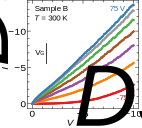
\includegraphics[width=4.9cm]{Chapter-In2Se3-FeSm-FET/Figures/JR200115_17/JR200115_17_300K_IDvVDS-negative_VG-increasing_linear_txt}\qquad{}
\par\end{flushright}%
\end{minipage}}
\par\end{centering}
\begin{centering}
\subfloat[$I_{D}\left(V_{DS,\uparrow},\,V_{G,\downarrow}\right)$\hfill{}]{\raggedleft{}%
\begin{minipage}[t]{0.3\paperwidth}%
\begin{flushright}
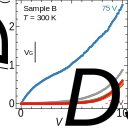
\includegraphics[width=4.37cm]{Chapter-In2Se3-FeSm-FET/Figures/JR200115_17/JR200115_17_300K_IDvVDS-positive_VG-decreasing_linear_txt}\qquad{}
\par\end{flushright}%
\end{minipage}}\quad{}\subfloat[$I_{D}\left(V_{DS,\downarrow},\,V_{G,\downarrow}\right)$\hfill{}]{\raggedleft{}%
\begin{minipage}[t]{0.3\paperwidth}%
\begin{flushright}
~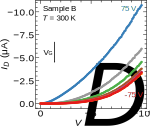
\includegraphics[width=5.2cm]{Chapter-In2Se3-FeSm-FET/Figures/JR200115_17/JR200115_17_300K_IDvVDS-negative_VG-decreasing_linear_txt}\qquad{}
\par\end{flushright}%
\end{minipage}}
\par\end{centering}
\caption{Sample B: $I_{D}\left(D_{DS},\,V_{G}\right)$ - linear scale\label{fig:Sample-B-IDvsVDS-linear}}

Linear graphs of figure \ref{fig:Sample-B-IDvsVDS-log}. $I_{D}\left(V_{DS}\right)$
of sample B with positive-increasing (a \& c) and negative-decreasing
(b \& d) $V_{DS}$. Measurements (a \& b) are taken while $V_{G}$
is held at 25 V intervals that increase sequentially for each curve,
and (c \& d) decreasing for $V_{G}$ intervals. All measurements were
done at 300 K.
\end{figure}

\noindent 
\begin{figure}
\begin{centering}
\subfloat[$I_{D}\left(V_{DS,\uparrow},\,V_{G,\uparrow}\right)$]{\raggedleft{}%
\begin{minipage}[t]{0.3\paperwidth}%
\begin{flushright}
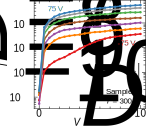
\includegraphics[width=5cm]{Chapter-In2Se3-FeSm-FET/Figures/JR190919_03/JR190919_03_300K_IDvVDS-positive_VG-increasing_log_txt}\qquad{}
\par\end{flushright}%
\end{minipage}}\quad{}\subfloat[$I_{D}\left(V_{DS,\downarrow},\,V_{G,\uparrow}\right)$\hfill{}]{\raggedleft{}%
\begin{minipage}[t]{0.3\paperwidth}%
\begin{flushright}
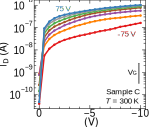
\includegraphics[width=5cm]{Chapter-In2Se3-FeSm-FET/Figures/JR190919_03/JR190919_03_300K_IDvVDS-negative_VG-increasing_log_txt}\qquad{}
\par\end{flushright}%
\end{minipage}}
\par\end{centering}
\begin{centering}
\subfloat[$I_{D}\left(V_{DS,\uparrow},\,V_{G,\downarrow}\right)$]{\raggedleft{}%
\begin{minipage}[t]{0.3\paperwidth}%
\begin{flushright}
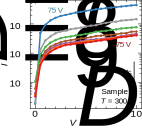
\includegraphics[width=5cm]{Chapter-In2Se3-FeSm-FET/Figures/JR190919_03/JR190919_03_300K_IDvVDS-positive_VG-decreasing_log_txt}\qquad{}
\par\end{flushright}%
\end{minipage}}\quad{}\subfloat[$I_{D}\left(V_{DS,\downarrow},\,V_{G,\downarrow}\right)$]{\raggedleft{}%
\begin{minipage}[t]{0.3\paperwidth}%
\begin{flushright}
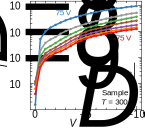
\includegraphics[width=5cm]{Chapter-In2Se3-FeSm-FET/Figures/JR190919_03/JR190919_03_300K_IDvVDS-negative_VG-decreasing_log_txt}\qquad{}
\par\end{flushright}%
\end{minipage}}
\par\end{centering}
\begin{centering}
\caption{Sample C: $I_{D}\left(V_{DS},\,V_{G}\right)$ - logarithmic scale\label{fig:Sample-C-IDvsVDS-log}}
\par\end{centering}
$I_{D}\left(V_{DS}\right)$ of sample C with positive-increasing (a
\& c) and negative-decreasing (b \& d) $V_{DS}$. Measurements (a
\& b) are taken while $V_{G}$ is held at 25 V intervals that increase
sequentially for each curve, and (c \& d) decreasing for $V_{G}$
intervals. All measurements were done at 300 K.
\end{figure}

\noindent 
\begin{figure}
\begin{centering}
\subfloat[$I_{D}\left(V_{DS,\uparrow},\,V_{G,\uparrow}\right)$\hfill{}]{\raggedleft{}%
\begin{minipage}[t]{0.3\paperwidth}%
\begin{flushright}
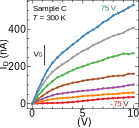
\includegraphics[width=5cm]{Chapter-In2Se3-FeSm-FET/Figures/JR190919_03/JR190919_03_300K_IDvVDS-positive_VG-increasing_linear_txt}\qquad{}
\par\end{flushright}%
\end{minipage}}\quad{}\subfloat[$I_{D}\left(V_{DS,\downarrow},\,V_{G,\uparrow}\right)$\hfill{}]{\raggedleft{}%
\begin{minipage}[t]{0.3\paperwidth}%
\begin{flushright}
~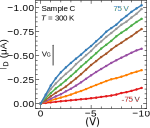
\includegraphics[width=5.26cm]{Chapter-In2Se3-FeSm-FET/Figures/JR190919_03/JR190919_03_300K_IDvVDS-negative_VG-increasing_linear_txt}\qquad{}
\par\end{flushright}%
\end{minipage}}
\par\end{centering}
\begin{centering}
\subfloat[$I_{D}\left(V_{DS,\uparrow},\,V_{G,\downarrow}\right)$\hfill{}]{\raggedleft{}%
\begin{minipage}[t]{0.3\paperwidth}%
\begin{flushright}
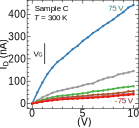
\includegraphics[width=5cm]{Chapter-In2Se3-FeSm-FET/Figures/JR190919_03/JR190919_03_300K_IDvVDS-positive_VG-decreasing_linear_txt}\qquad{}
\par\end{flushright}%
\end{minipage}}\quad{}\subfloat[$I_{D}\left(V_{DS,\downarrow},\,V_{G,\downarrow}\right)$\hfill{}]{\raggedleft{}%
\begin{minipage}[t]{0.3\paperwidth}%
\begin{flushright}
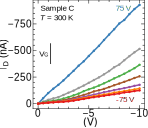
\includegraphics[width=5.2cm]{Chapter-In2Se3-FeSm-FET/Figures/JR190919_03/JR190919_03_300K_IDvVDS-negative_VG-decreasing_linear_txt}\qquad{}
\par\end{flushright}%
\end{minipage}}
\par\end{centering}
\caption{Sample C: $I_{D}\left(V_{DS},\,V_{G}\right)$- linear scale\label{fig:Sample-C-IDvsVDS-linear}}

Linear graphs of figure \ref{fig:Sample-C-IDvsVDS-log}.$I_{D}\left(V_{DS}\right)$
of sample C with positive-increasing (a \& c) and negative-decreasing
(b \& d) $V_{DS}$. Measurements (a \& b) are taken while $V_{G}$
is held at 25 V intervals that increase sequentially for each curve,
and (c \& d) decreasing for $V_{G}$ intervals. All measurements were
done at 300 K.
\end{figure}

\noindent 
\begin{figure}
\begin{centering}
\subfloat[300 K]{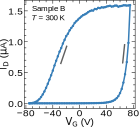
\includegraphics[width=5cm]{Chapter-In2Se3-FeSm-FET/Figures/JR200115_17/JR200115_17_IDvVG_300K_log_txt}}~\subfloat[250 K]{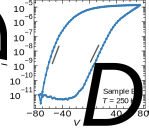
\includegraphics[width=5cm]{Chapter-In2Se3-FeSm-FET/Figures/JR200115_17/JR200115_17_IDvVG_250K_log_txt}}~\subfloat[200 K]{\includegraphics[width=5cm]{Chapter-In2Se3-FeSm-FET/Figures/JR200115_17/JR200115_17_IDvVG_200K_log_txt}}
\par\end{centering}
\begin{centering}
\subfloat[150 K]{\includegraphics[width=5cm]{Chapter-In2Se3-FeSm-FET/Figures/JR200115_17/JR200115_17_IDvVG_150K_log_txt}

}~\subfloat[100 K]{\includegraphics[width=5cm]{Chapter-In2Se3-FeSm-FET/Figures/JR200115_17/JR200115_17_IDvVG_100K_log_txt}}~\subfloat[50 K]{\includegraphics[width=5cm]{Chapter-In2Se3-FeSm-FET/Figures/JR200115_17/JR200115_17_IDvVG_050K_log_txt}}
\par\end{centering}
\begin{centering}
\subfloat[3 K]{~\includegraphics[width=5cm]{Chapter-In2Se3-FeSm-FET/Figures/JR200115_17/JR200115_17_IDvVG_003K_log_txt}

}
\par\end{centering}
\caption{Sample B: $I_{D}\left(V_{G}\right)$ transfer characteristics\label{fig:Sample-B-loops}}

$I_{D}\left(V_{G}\right)$ of sample B at the indicated fixed temperatures.
Each was measured with $V_{DS}=0.1\,V$ as $V_{G}$ was cycled, a
clockwise hysteresis loop was seen at all temperatures.
\end{figure}

\noindent 
\begin{figure}
\begin{centering}
\subfloat[300 K]{\includegraphics[width=5cm]{Chapter-In2Se3-FeSm-FET/Figures/JR190919_03/JR190919_03_IDvVG_300K_log_txt}}~~\subfloat[250 K]{\includegraphics[width=5cm]{Chapter-In2Se3-FeSm-FET/Figures/JR190919_03/JR190919_03_IDvVG_250K_log_txt}}~~\subfloat[200 K]{\includegraphics[width=5cm]{Chapter-In2Se3-FeSm-FET/Figures/JR190919_03/JR190919_03_IDvVG_200K_log_txt}}
\par\end{centering}
\begin{centering}
\subfloat[150 K]{\includegraphics[width=5cm]{Chapter-In2Se3-FeSm-FET/Figures/JR190919_03/JR190919_03_IDvVG_150K_log_txt}}~~\subfloat[100 K]{\includegraphics[width=5cm]{Chapter-In2Se3-FeSm-FET/Figures/JR190919_03/JR190919_03_IDvVG_100K_log_txt}}~~\subfloat[50 K]{\includegraphics[width=5cm]{Chapter-In2Se3-FeSm-FET/Figures/JR190919_03/JR190919_03_IDvVG_050K_log_txt}

}
\par\end{centering}
\begin{centering}
\subfloat[20 K]{~~~~~~~~\includegraphics[width=5cm]{Chapter-In2Se3-FeSm-FET/Figures/JR190919_03/JR190919_03_IDvVG_020K_log_txt}}~~\subfloat[4 K]{\includegraphics[width=5cm]{Chapter-In2Se3-FeSm-FET/Figures/JR190919_03/JR190919_03_IDvVG_004K_log_txt}}
\par\end{centering}
\caption{Sample C: $I_{D}\left(V_{G}\right)$ transfer characteristics\label{fig:Sample-C-loops}}

$I_{D}\left(V_{G}\right)$ of sample C at the indicated fixed temperatures.
Each was measured with $V_{DS}=0.1\,V$ as $V_{G}$ was cycled, a
clockwise hysteresis loop was seen at all temperatures.
\end{figure}

\noindent 
\begin{figure}
\begin{centering}
\subfloat[250 K]{\includegraphics[width=5cm]{Chapter-In2Se3-FeSm-FET/Figures/JR190815_04/JR190815_04_11_IDvVG_250K_log_txt}}~~\subfloat[150 K]{\includegraphics[width=5cm]{Chapter-In2Se3-FeSm-FET/Figures/JR190815_04/JR190815_04_11_IDvVG_150K_log_txt}}~~\subfloat[100 K]{\includegraphics[width=5cm]{Chapter-In2Se3-FeSm-FET/Figures/JR190815_04/JR190815_04_11_IDvVG_100K_log_txt}}
\par\end{centering}
\begin{centering}
\subfloat[50 K]{\includegraphics[width=5cm]{Chapter-In2Se3-FeSm-FET/Figures/JR190815_04/JR190815_04_11_IDvVG_050K_log_txt}}~~\subfloat[4 K]{\includegraphics[width=5cm]{Chapter-In2Se3-FeSm-FET/Figures/JR190815_04/JR190815_04_11_IDvVG_004K_log_txt}}~~\subfloat[$R_{DS}\left(T\right)$]{\includegraphics[width=5cm]{Chapter-In2Se3-FeSm-FET/Figures/JR190815_04/JR190815_04_RDSvVG-cross-section_log}

}
\par\end{centering}
\caption{Sample D: $I_{D}\left(V_{G}\right)$ transfer characteristics\label{fig:Sample-D-loops}}

(a-e) $I_{D}\left(V_{G}\right)$ of sample D at the indicated fixed
temperatures. Each was measured with $V_{DS}=0.1\,V$ as $V_{G}$
was cycled, a clockwise hysteresis loop was seen at all temperatures.
(f) Temperature cross-section of the $I_{D}\left(V_{G}\right)$ transfer
characteristics. Each data-point is taken from the increasing $V_{G}$
(top) portion of the respective $I_{D}\left(V_{G}\right)$ curves
for 0, 25, 50, and 75 V.
\end{figure}

\noindent 
\begin{figure}
\begin{centering}
\subfloat[10 \textgreek{m}A]{\begin{centering}
\includegraphics[width=4.8cm]{Chapter-In2Se3-FeSm-FET/Figures/Devices/Devices_DVGvT_10uA}
\par\end{centering}
}~~\subfloat[1 \textgreek{m}A]{\begin{centering}
\includegraphics[width=4.8cm]{Chapter-In2Se3-FeSm-FET/Figures/Devices/Devices_DVGvT_1uA}
\par\end{centering}
}~~\subfloat[100 nA]{\begin{centering}
\includegraphics[width=4.8cm]{Chapter-In2Se3-FeSm-FET/Figures/Devices/Devices_DVGvT_100nA}
\par\end{centering}
}
\par\end{centering}
\begin{centering}
\subfloat[10 nA]{\begin{centering}
\includegraphics[width=4.8cm]{Chapter-In2Se3-FeSm-FET/Figures/Devices/Devices_DVGvT_10nA}
\par\end{centering}
}~~\subfloat[1 nA]{\begin{centering}
\includegraphics[width=4.8cm]{Chapter-In2Se3-FeSm-FET/Figures/Devices/Devices_DVGvT_1nA}
\par\end{centering}
}~~\subfloat[100 pA]{\begin{centering}
\includegraphics[width=4.8cm]{Chapter-In2Se3-FeSm-FET/Figures/Devices/Devices_DVGvT_100pA}
\par\end{centering}
}
\par\end{centering}
\begin{centering}
\subfloat[Threshold voltage, $\Delta V_{T}$]{\includegraphics[width=4.8cm]{Chapter-In2Se3-FeSm-FET/Figures/Devices/Devices_DVTvT}

}
\par\end{centering}
\caption{Hysteresis width $\Delta V_{G}$ versus temperature for samples A,
B, C, and D\label{fig:dVG-vs-T}}

The width of the gate voltage hysteresis versus temperatures for all
four sample devices. (a-f) shows the width for different current levels,
in multiples of 10. Values found using the data shown in figures (Sample)
\ref{fig:In2Se3-Sample-A-loops} (A), \ref{fig:Sample-B-loops} (B),
\ref{fig:Sample-C-loops} (C), and \ref{fig:Sample-D-loops} (D).
(g) hysteresis width of the threshold voltage for the four samples.
The threshold voltage was found by separately fitting the increasing
and decreasing linear voltage regions\citep{2013revisiting}. Sample
D data was excluded at higher temperatures due to noise or too few
points in the linear region to fit well.
\end{figure}

\noindent 
\begin{figure}
\begin{centering}
\subfloat[Sample A]{\includegraphics[width=5cm]{Chapter-In2Se3-FeSm-FET/Figures/JR200115_11/JR200115_11_minSSvsT}

}~~\subfloat[Sample B]{\includegraphics[width=5cm]{Chapter-In2Se3-FeSm-FET/Figures/JR200115_17/JR200115_17_minSSvsT}

}
\par\end{centering}
\begin{centering}
\subfloat[Sample C]{\includegraphics[width=5cm]{Chapter-In2Se3-FeSm-FET/Figures/JR190919_03/JR190919_03_minSSvsT}

}~~\subfloat[Sample D]{\includegraphics[width=5cm]{Chapter-In2Se3-FeSm-FET/Figures/JR190815_04/JR190815_04_minSSvsT}

}
\par\end{centering}
\caption{Minimum subthreshold slope (SS) versus temperature\label{fig:Min-subthreshold-slope-vs-T}}

The minimum threshold slope for increasing and decreasing gate voltage
sweeps. Maximum slope (minimum SS) was found for five data points
for measurements shown in in figures (Sample) \ref{fig:In2Se3-Sample-A-loops}
(A), \ref{fig:Sample-B-loops} (B), \ref{fig:Sample-C-loops} (C),
and \ref{fig:Sample-D-loops} (D). Calculated values are all well
above the Boltzman limit threshold\citep{beckers2018cryogenic}, which
about 60 mV/dec at 300 K, values below the limit are often used as
a sign the hysteresis is an effect of polarization switching instead
of charge trapping\citep{jin2019onthe,jin2020physical}. All slopes
were calculated using $SS=1/\frac{\partial\log_{10}I_{D}}{\partial V_{G}}$.
\end{figure}

\noindent 
\begin{figure}
\begin{centering}
\subfloat[two-point]{\includegraphics[width=5cm]{Chapter-In2Se3-FeSm-FET/Figures/JR190919_03/JR190919_03_RDSvT_warming-after-VG-cooled}}~\subfloat[four-point]{\includegraphics[width=5cm]{Chapter-In2Se3-FeSm-FET/Figures/JR190919_03/JR190919_03_R4PTvT_warming-after-VG-cooled}}~\subfloat[Cooling vs warming]{\includegraphics[width=5.2cm]{Chapter-In2Se3-FeSm-FET/Figures/JR190919_03/JR190919_03_IDvT_cooling-vs-warming-at-VG-75V}}
\par\end{centering}
\caption{Sample C: effects of warming and cooling while gated\label{fig:Sample-C-effects-of-warming-cooling}}

Sample C (a) two-point and (b) four-point resistance measured at $V_{G}=75\,V$
with increasing temperature from 2 to 300 K. Before each measurement,
sample were cycled at 300 K to $V_{G}=-75\,V$, then fixed at 25,
50, and 75 V as indicated, then finally cooled from 300 to 2 K with
the $V_{G}$ still held constant. (c) Sample was cycled at 2 K (300
K) to $V_{G}=-75\,\mathrm{V}$ then to 75 V and held fixed. $I_{D}$
was measured while sample was warmed (cooled) with constant $V_{G}$
and $V_{DS}=1\,\mathrm{V}$.
\end{figure}

\noindent 
\begin{figure}
\begin{centering}
\subfloat[300 K]{\includegraphics[width=5cm]{Chapter-In2Se3-FeSm-FET/Figures/JR200115_17/JR200115_17_IDvVG-rate_300K_log}

}~~\subfloat[3 K]{\includegraphics[width=5cm]{Chapter-In2Se3-FeSm-FET/Figures/JR200115_17/JR200115_17_IDvVG-rate_3K_log}

}
\par\end{centering}
\caption{Sample B: $I_{D}\left(V_{G}\right)$, $V_{G}$ rate dependence\label{fig:Sample-B-rate-dependance}}

$I_{D}\left(V_{G}\right)$ of sample C taken at (a) 300 K and (b)
3 K. Each curve was taken with $V_{G}$ increased and decreased at
the indicated rate with $V_{DS}=0.1\,V$.
\end{figure}

\noindent 
\begin{figure}
\begin{centering}
\includegraphics[width=5.2cm]{Chapter-In2Se3-FeSm-FET/Figures/JR190815_04/JR190815_04_RvVG_300K_contact-and-sample}
\par\end{centering}
\caption{Sample D: contact resistance\label{fig:Sample-D-contact-resistance}}

Sample D $R\left(V_{G}\right)$ contact and four-point sample resistance,
taken at 300 K with increasing $V_{G}$.
\end{figure}

\noindent 
\begin{figure}
\begin{centering}
\subfloat[Sample C: $I_{D}\left(V_{DS}\right)$]{\includegraphics[width=5cm]{Chapter-In2Se3-FeSm-FET/Figures/JR190919_03/JR190919_03_IDvVDS_effect-of-heating_linear}

}~~\subfloat[Sample C: $I_{D}\left(V_{G}\right)$]{\includegraphics[width=4.9cm]{Chapter-In2Se3-FeSm-FET/Figures/JR190919_03/JR190919_03_IDvVG_effect-of-heating_linear}

}~~\subfloat[Sample B: $I_{D}\left(V_{G}\right)$]{\includegraphics[width=5.31cm]{Chapter-In2Se3-FeSm-FET/Figures/JR200115_17/JR200115_17_IDvVG_effect-of-heating_log}

}
\par\end{centering}
\caption{Sample A and B: annealing\label{fig:Sample-AB-Annealing}}

Samples A (a \& b) and B (c) were annealed in vacuum at 400 K in 1
hour intervals. (a) Show $I_{D}\left(V_{DS}\right)$ measurements
and (b \& c) $I_{D}\left(V_{G}\right)$, each taken at 300 K.
\end{figure}

